\section{Computational Platforms and Software Libraries}
This section describes technical details about the implementation of the solutions exposed in this document. It also contains
the collected data used for the analysis.

The results of each run are tested with 16bit Fletcher's checksum so that errors can be quickly checked over large matrices \cite{fletcher}.
\subsection{Serial implementation}
The \emph{sequential} version of the FW algorithm can be found \href{https://github.com/firaja/Parallel-FloydWarshall/blob/master/sequential.c}{here}. 
The program is compiled as follows:
\begin{lstlisting}[basicstyle=\footnotesize\ttfamily]
$ gcc sequential.c -o sequential.out -O3
\end{lstlisting}

notice the \texttt{-O3} flag that makes the program run $3.5$ times faster.
The program accepts 2 arguments:
\begin{lstlisting}[basicstyle=\footnotesize\ttfamily]
$ ./sequential.out <v> <d>
\end{lstlisting}
where \texttt{v} is the number of verteces, expressed as positive integer, and \texttt{d} is the density of the presence of edges, expressed as an integer from 0 to 100.
\par
The \texttt{gcc} version used for this work is 7.5.0 and the program ran on a Intel Core i7-9700K. \\
\textbf{Table \ref*{tab:seq-time}} shows the execution time (expressed in milliseconds) depending on the number of vertices.


\begin{table}[h!]
\centering
\begin{tabular}{|r|r|}
\hline
\rowcolor[HTML]{3166FF} 
{\color[HTML]{FFFFFF} \textbf{Vertices}} & {\color[HTML]{FFFFFF} \textbf{Execution time}} \\ \hline
1000                                     & 1095 ms                                        \\ \hline
2000                                     & 8860 ms                                        \\ \hline
5000                                     & 138643 ms                                      \\ \hline
7500                                     & 468750 ms                                      \\ \hline
10000                                    & 1112111 ms                                     \\ \hline
12500                                    & 2170138 ms                                     \\ \hline
\end{tabular}
\caption{Execution time of the \emph{serial} FW}                                                                                                                                            
\label{tab:seq-time} 
\end{table}

\textbf{Figure \ref*{fig:seq-time}} shows the trend of the execution time. 

\begin{figure}[h!]
\centering                                                                        
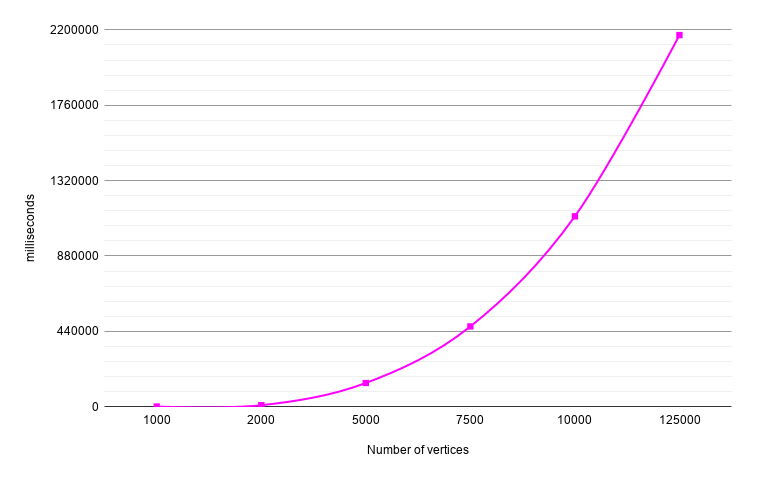
\includegraphics[width=3.5in]{images/seq-time}
\captionsetup{justification=centering,margin=2cm}                                                                                                                                   
\caption{Trend of the execution time based on Table \ref*{tab:seq-time}}                                                                                                                                            
\label{fig:seq-time}                                                                                                                                                           
\end{figure}


It is easy to notice that the graph represents a 
third grade curve; this is the interpolated function starting from the collected data:
\[f(n) = 2.22n^3 - 18.83n^2 + 92.14n -94.84 \in \Theta(n^3) \]



\subsection{MPI implementation}

The \emph{MPI} version of the FW algorithm can be found \href{https://github.com/firaja/Parallel-FloydWarshall/blob/master/mpi.c}{here}. 
The program is compiled as it follows:

\begin{lstlisting}[basicstyle=\footnotesize\ttfamily]
$ mpicc -g -Wall mpi.c -o mpi.out -O3
\end{lstlisting}
Like the \emph{serial} version, the program accepts 2 arguments + 1 for $\texttt{mpirun}$:
\begin{lstlisting}[basicstyle=\footnotesize\ttfamily]
$ mpirun -np <p> mpi.out <v> <d>
\end{lstlisting}
The \texttt{MPI} version used for this work is 2.1.1 and the program ran on a cluster of 8 nodes over a LAN. \\
\textbf{Table \ref*{tab:mpi-time}} shows the execution time (expressed in milliseconds) and the percentage of time spent in initialization and communication, depending on the number of processors; 
in this case the program computed the \emph{APSP} problem for 5040 vertices.

\begin{table}[h!]
\centering
\begin{tabular}{|r|r|r|}
\hline
\rowcolor[HTML]{F56B00} 
{\color[HTML]{FFFFFF} \textbf{Processors}} & {\color[HTML]{FFFFFF} \textbf{Execution time}} & {\color[HTML]{FFFFFF} \textbf{MPI \%}} \\ \hline
1                                          & 145447 ms                                               & 0.06                                 \\ \hline
2                                          & 75059 ms                                               & 2.57                                 \\ \hline
3                                          & 52336 ms                                               & 4.45                                \\ \hline
4                                          & 39962 ms                                               & 5.47                                \\ \hline
5                                          & 33184 ms                                               & 6.95                                 \\ \hline
6                                          & 28731 ms                                               & 8.35                                \\ \hline
7                                          & 25853 ms                                               & 9.50                                 \\ \hline
8                                          & 23120 ms                                               & 11.00                                \\ \hline
\end{tabular}
\caption{Execution time of the \emph{MPI} FW}                                                                                                                                            
\label{tab:mpi-time}
\end{table}
Timings are captured through \texttt{mpiP} that calculates the percentage of time spent by MPI for initialization/finalization and communication.
\texttt{mpiP} is a lightweight profiling library for MPI applications. Because it only collects statistical information about MPI functions, \texttt{mpiP} generates considerably less overhead and much less data than tracing tools. All the information captured by mpiP is task-local. It only uses communication during report generation, typically at the end of the experiment, to merge results from all of the tasks into one output file.


\subsection{OpenMP implementation}
The \emph{OpenMP} version of the FW algorithm can be found \href{https://github.com/firaja/Parallel-FloydWarshall/blob/master/openmp.c}{here}. 
The program is compiled as it follows:
\begin{lstlisting}[basicstyle=\footnotesize\ttfamily]
$ g++ -fopenmp openmp.c -o openmp.out -O3
\end{lstlisting}
Unlike the \emph{serial} version, the program accepts 3 arguments:
\begin{lstlisting}[basicstyle=\footnotesize\ttfamily]
$ ./openmp.out <v> <d> <t>
\end{lstlisting}
where \texttt{t} is the number of threads OpenMP can use for parallelization. \\
The \texttt{gcc} version used for this work is 7.5.0 and the program ran on a Intel Core i7-9700K, which has 8 core with no Hyper-Threading.
\textbf{Table \ref*{tab:omp-time}} shows the execution time (expressed in milliseconds) depending on the number of vertices and available cores.

\begin{table}[h!]
\centering
\begin{tabular}{|r|r|r|r|}
\hline
\rowcolor[HTML]{CB0000} 
\multicolumn{1}{|c|}{\cellcolor[HTML]{CB0000}{\color[HTML]{FFFFFF} \textbf{Vertices}}} & \multicolumn{1}{c|}{\cellcolor[HTML]{CB0000}{\color[HTML]{FFFFFF} \textbf{2 threads}}} & \multicolumn{1}{c|}{\cellcolor[HTML]{CB0000}{\color[HTML]{FFFFFF} \textbf{4 threads}}} & \multicolumn{1}{c|}{\cellcolor[HTML]{CB0000}{\color[HTML]{FFFFFF} \textbf{8 threads}}} \\ \hline
1000                                                                                   & 541 ms                                                                                         & 364 ms                                                                                         & 158 ms                                                                                          \\ \hline
2000                                                                                   & 4365 ms                                                                                        & 2921 ms                                                                                        & 1260 ms                                                                                         \\ \hline
5000                                                                                   & 69590 ms                                                                                       & 46443 ms                                                                                       & 19496 ms                                                                                        \\ \hline
7500                                                                                   & 230260 ms                                                                                      & 155531 ms                                                                                      & 65118 ms                                                                                        \\ \hline
10000                                                                                  & 543900 ms                                                                                      & 367434 ms                                                                                       & 153682 ms                                                                                       \\ \hline
12500                                                                                  & 1063129 ms                                                                                     & 716363 ms                                                                                       & 299006 ms                                                                                       \\ \hline
\end{tabular}
\caption{Execution time of the \emph{OpenMP} FW}                                                                                                                                            
\label{tab:omp-time}
\end{table}

\subsection{CUDA implementation}
The \emph{CUDA} version of the FW algorithm can be found \href{https://github.com/firaja/Parallel-FloydWarshall/blob/master/cuda.cu}{here}. Alternatively the version 
that uses only global memory is \href{https://github.com/firaja/Parallel-FloydWarshall/blob/master/cuda2.cu}{here}.
The program is compiled as follows:
\begin{lstlisting}[basicstyle=\footnotesize\ttfamily]
$ nvcc cuda.cu -o cuda.out \
  -gencode=arch=compute_75,code=compute_75 -O3
\end{lstlisting}
Unlike the \emph{serial} version, the program accepts 3 arguments:
\begin{lstlisting}[basicstyle=\footnotesize\ttfamily]
$ ./cuda.out <v> <d> <b>
\end{lstlisting}
where \texttt{b} is the number of threads per block. \\
The \texttt{nvcc} version used for this work is 10.2 and the program ran on a CPU Intel Core i7-9700K and a GPU NVIDIA GeForce RTX 2070 Super.
Table \ref*{tab:cuda-time} shows the execution time (expressed in milliseconds) depending on the number of vertices and the block size of threads.

\begin{table}[h!]
\centering
\begin{tabular}{|r|r|r|r|}
\hline
\rowcolor[HTML]{009901} 
\multicolumn{1}{|l|}{\cellcolor[HTML]{009901}{\color[HTML]{FFFFFF} \textbf{verteces}}} & \multicolumn{1}{l|}{\cellcolor[HTML]{009901}{\color[HTML]{FFFFFF} \textbf{1024 block}}} & {\color[HTML]{FFFFFF} \textbf{256 block}} & \multicolumn{1}{l|}{\cellcolor[HTML]{009901}{\color[HTML]{FFFFFF} \textbf{32 block}}} \\ \hline
1000                                                                                   & 24 ms                                                                                                & 19 ms                                                  & 53 ms                                                                                              \\ \hline
2000                                                                                   & 219 ms                                                                                               & 186 ms                                                 & 356 ms                                                                                            \\ \hline
5000                                                                                   & 2818 ms                                                                                              & 2709 ms                                                & 4966 ms                                                                                            \\ \hline
7500                                                                                   & 9894 ms                                                                                              & 9044 ms                                                & 16297 ms                                                                                           \\ \hline
10000                                                                                  & 22190 ms                                                                                             & 21392 ms                                               & 38208 ms                                                                                           \\ \hline
125000                                                                                 & 42955 ms                                                                                             & 41460 ms                                               & 75034 ms                                                                                           \\ \hline
\end{tabular}
\caption{Execution time of the \emph{CUDA} FW}                                                                                                                                            
\label{tab:cuda-time}
\end{table}


Using a CPU-based timer would measure only the kernel's launch time and not the kernel's execution time and it would require a host-device synchronization point, like \texttt{cudaDeviceSynchronize()} which stalls the GPU pipeline.

So timings are taken with CUDA events that are created and destroyed with \texttt{cudaEventCreate()} and \texttt{cudaEventDestroy()}. \texttt{cudaEventRecord()} places the start and stop events into the default stream  and the device will record a time stamp for the event when it reaches that event in the stream. 
The \texttt{cudaEventElapsedTime()} function returns in the first argument the number of milliseconds time elapsed between the recording events. This value has a resolution of approximately one half microsecond.







